\chapter{Coil array WPT}\chaplab{result}
% 通过上一章节的讲解,我们知道了无线传输系统在水下的基本表现。这章将介绍我们设计出的水下线圈组wpt系统,通过将大型的双线圈结构降解为多个小线圈结构,这使得内部线圈里面的磁场大幅减小,从而实现对AUV系统内部的电磁保护。
Through the explanation in the previous chapter, we know the basic performance of the wireless transmission system underwater. This chapter will introduce the underwater coil-array WPT system we designed, by degrading a large double coil structure into multiple small coil structures, as shown in figure \ref{fig:3_coil_array_structure}. This greatly reduces the magnetic field in the internal coil, thereby achieving electromagnetic protection inside the AUV system. Its detailed parameters are shown in table 1.

\begin{figure}[htbp]
    \centering
    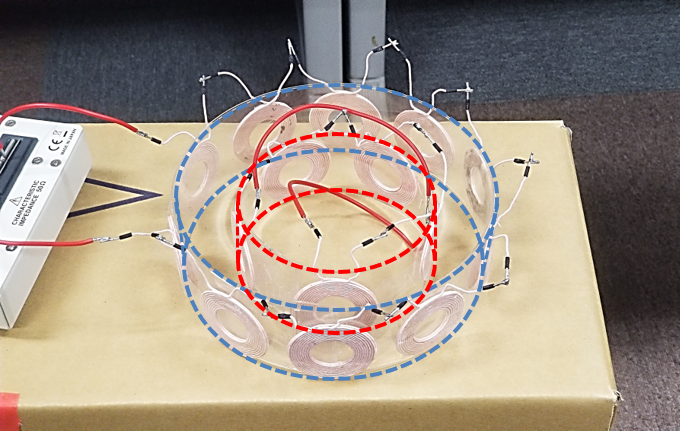
\includegraphics[width=0.7\linewidth]{images/3_coil_array_structure.png}
    \caption{Coil-array structure.}
    \label{fig:3_coil_array_structure}
\end{figure}

% 参数表格
\begin{table}[htbp]
    \centering
    \caption{The parameters of coil-array structure.}
    \begin{tabular}{ c|cc }
        \thickhline
        % \hline
        \textbf{Items}                    & \textbf{Parameters}      \\
        \thickhline
      
        Tx coil diameter                  & 113mm                    \\ \hline
        Rx coil diameter                  & 85mm                     \\ \hline
        Turns (Inner coil and outer coil) & 10                       \\ \hline
        Frequency                         & 200kHz                   \\ \hline
    \end{tabular}
    \label{table: coil array parameters}
\end{table}

In the marine environment, we can use buoys to generate electricity \cite{Orekan}, store the collected electricity in the power source, and then connect the power source to the transmitter (Tx). When the AUV reaches the designated position of transmitter, the AUV can be charged wirelessly.
Figure \ref{fig:3_coil_array_uwpt} shows a schematic diagram of the UWPT system.
\begin{figure}[htbp]
    \centering
    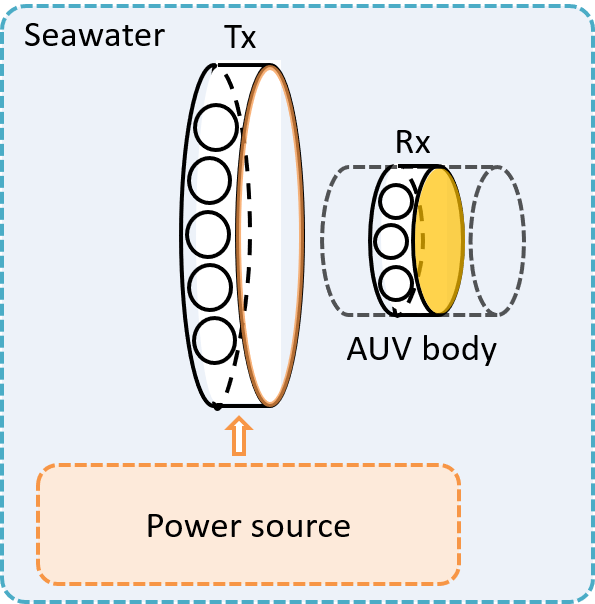
\includegraphics[width=0.5\linewidth]{images/3_coil_array_uwpt.png}
    \caption{Sechematic diagram of coil-array UWPT system.}
    \label{fig:3_coil_array_uwpt}
\end{figure}

% \begin{figure}[htbp]
%     \centering
%     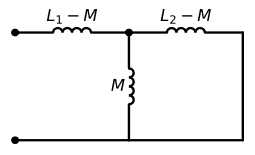
\includegraphics{images/3_mutual_inductance.png}
%     \caption{svg image}
% \end{figure}

\section{Simulation evaluation}


\begin{figure}[htbp]
    \begin{subfigure}{0.5\textwidth}
        \centering
        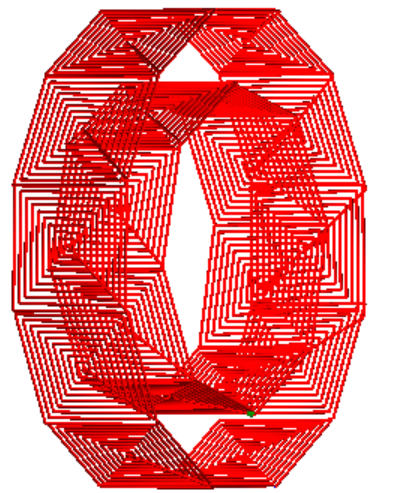
\includegraphics[height=6.4cm]{images/4_coil_array_system.png}
    \caption{Coil-array IPT structure.}
        \label{fig:subim1}
    \end{subfigure}
    \begin{subfigure}{0.5\textwidth}
        \centering
        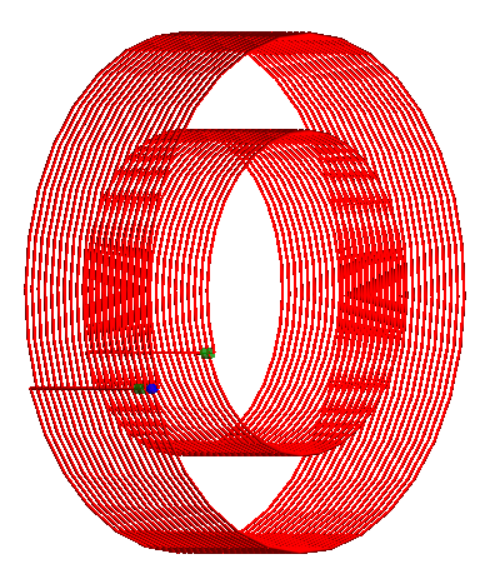
\includegraphics[height=6.4cm]{images/4_two_ring_system.png}
    \caption{Two ring IPT structure.}
        \label{fig:subim2}
    \end{subfigure}

    \caption{Two kind of UWPT coil structure simulation diagram.}
    \label{fig:3_two_ring_coil}
\end{figure}


\begin{figure}[htbp]
    \centering
    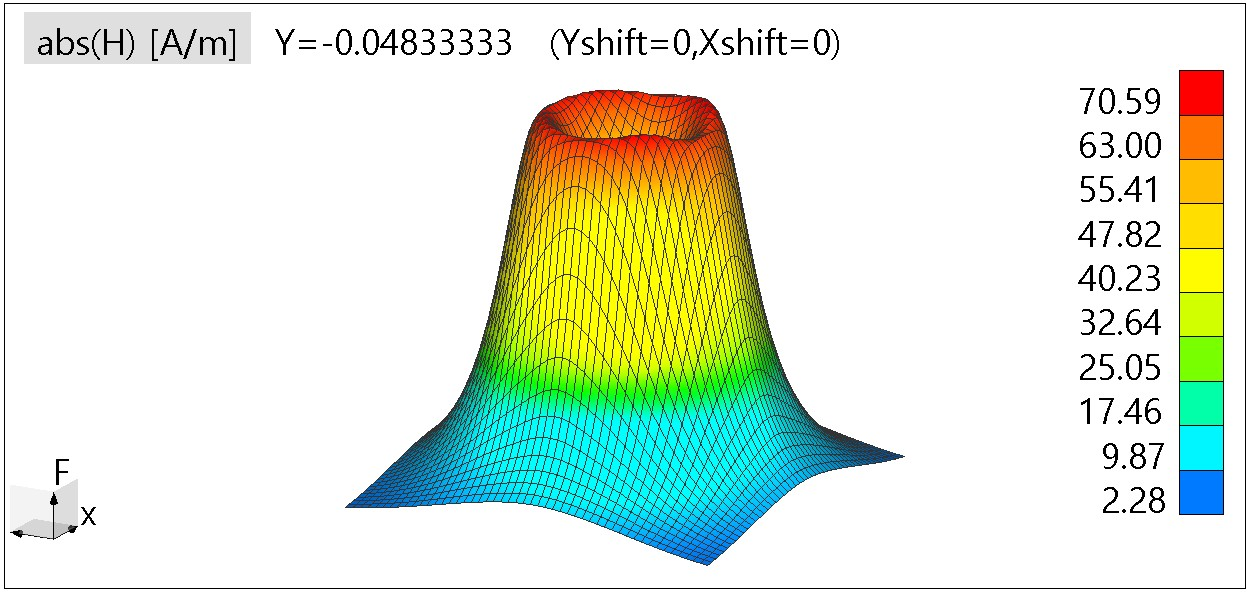
\includegraphics[width=0.9\linewidth]{images/4_coil_array_near_field_distribution.JPG}
    \caption{Magnetic field distribution of coil-array IPT structure.}
\end{figure}

\begin{figure}[htbp]
    \centering
    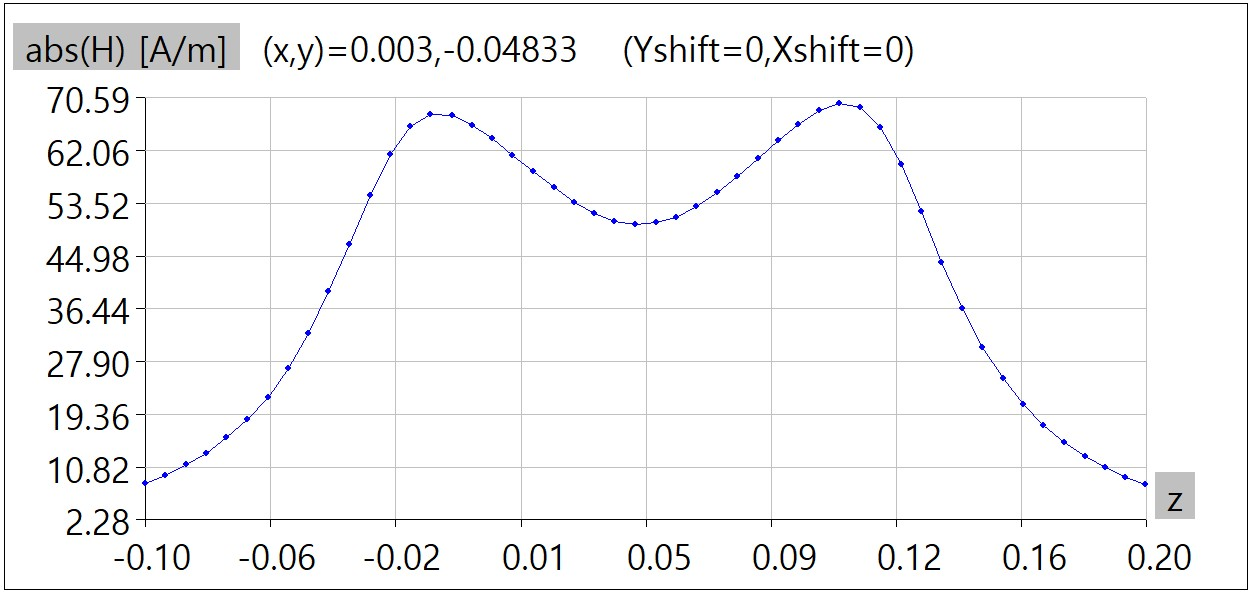
\includegraphics[width=0.9\linewidth]{images/4_coil_array_near_field_distribution_cut.JPG}
    \caption{Cross-sectional view of the magnetic field distribution of aoil-array IPT structure.}
\end{figure}

\begin{figure}[htbp]
    \centering
    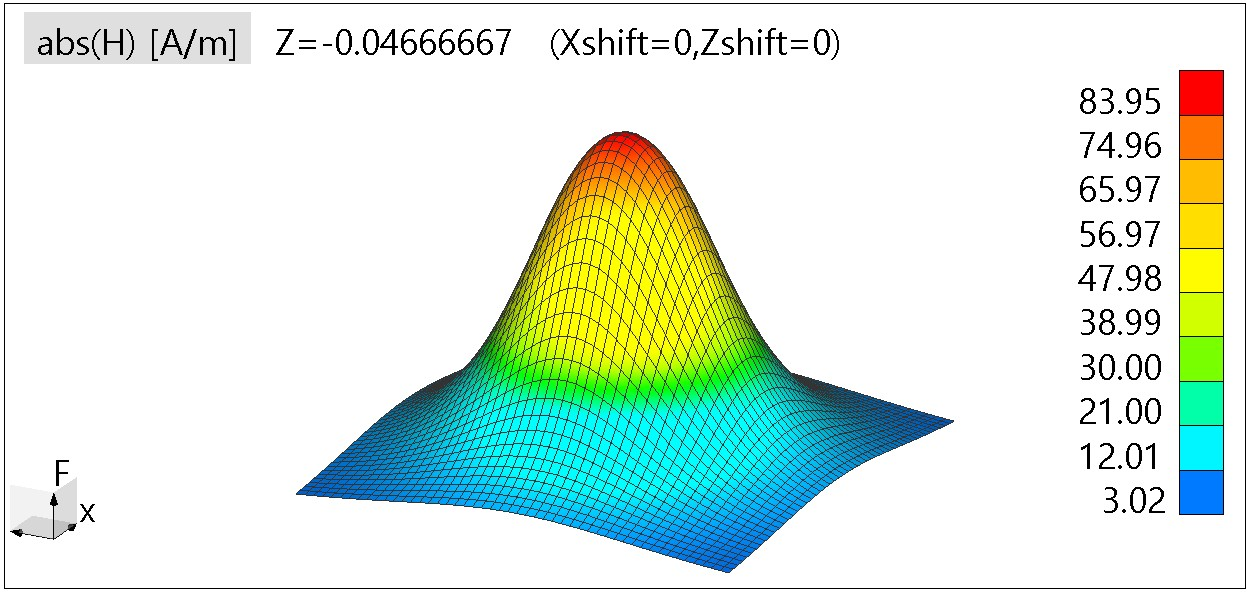
\includegraphics[width=0.9\linewidth]{images/4_two_ring_near_field_distribution.JPG}
    \caption{Magnetic field distribution of two ring IPT structure.}
\end{figure}

\begin{figure}[htbp]
    \centering
    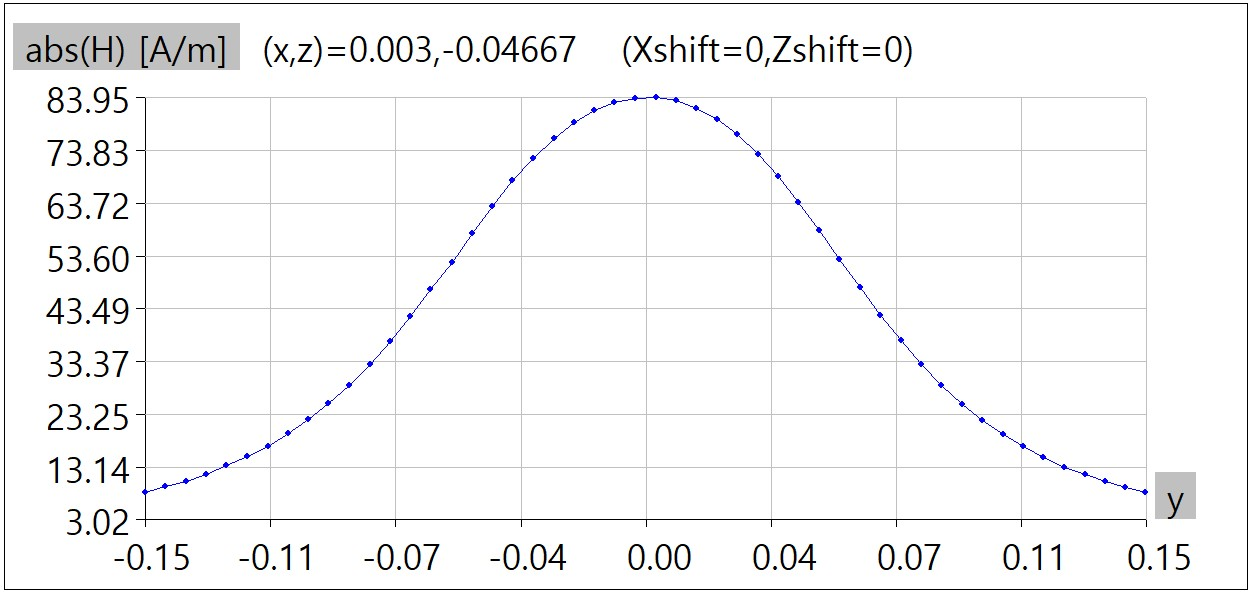
\includegraphics[width=0.9\linewidth]{images/4_two_ring_near_field_distribution_cut.JPG}
    \caption{Cross-sectional view of the magnetic field distribution of two ring IPT structure.}
\end{figure}

% 改变内部线圈的偏移,双方向下的偏移。

\subsection{Simulation evaluation}


\section{Coil array WPT in the air}
\begin{figure}[htbp]
    \centering
    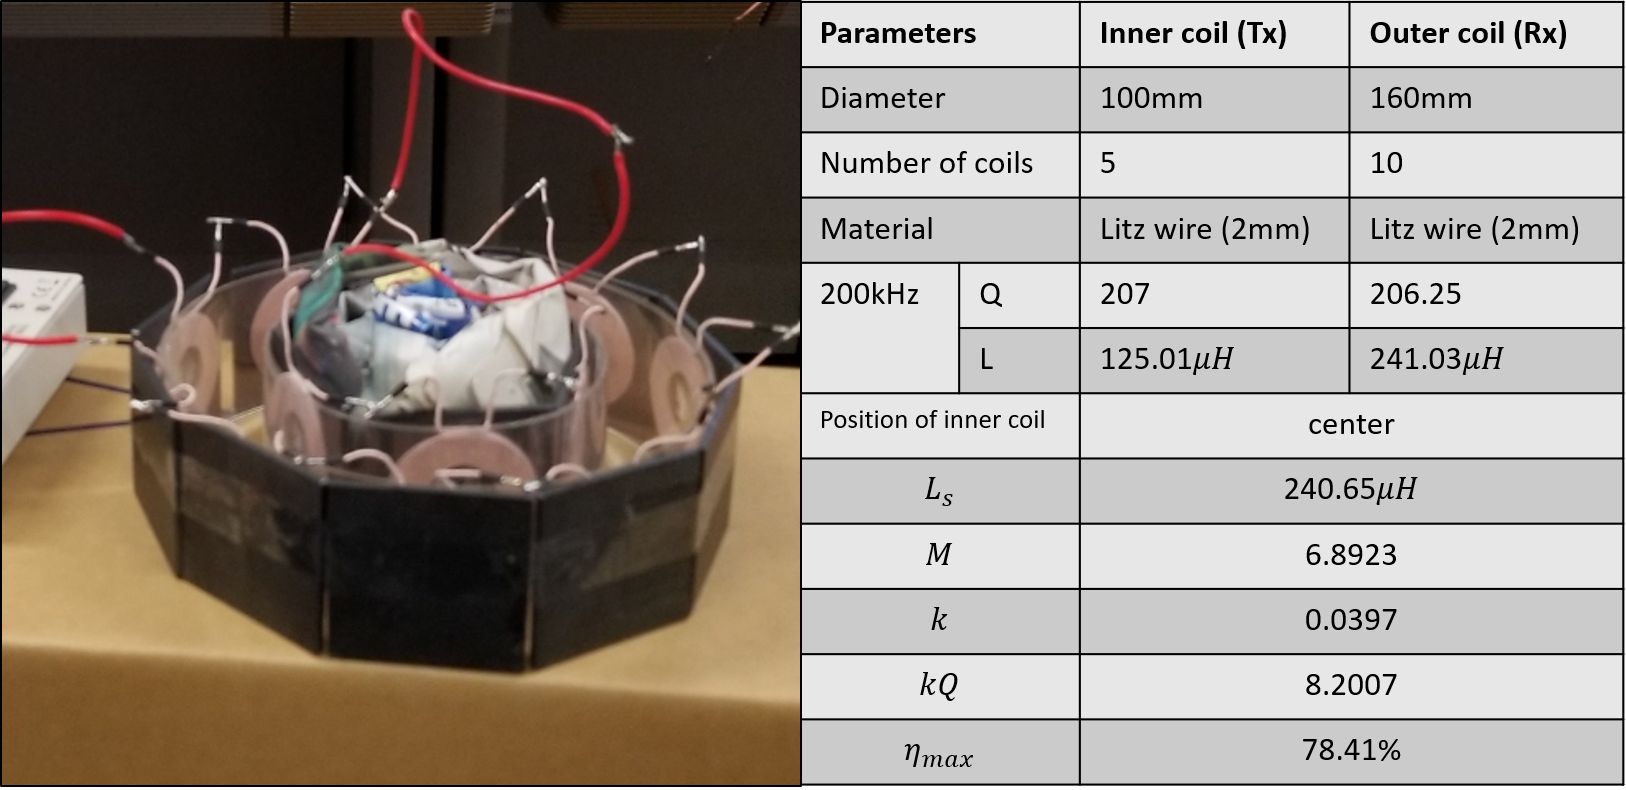
\includegraphics[width=1.0\linewidth]{images/4_coil_5_10_with_ferrite.png}
    \caption{Coil-array IPT structure (Both sides with ferrite tile), inner coil in the center or the outer coil.}
\end{figure}
\begin{figure}[htbp]
    \centering
    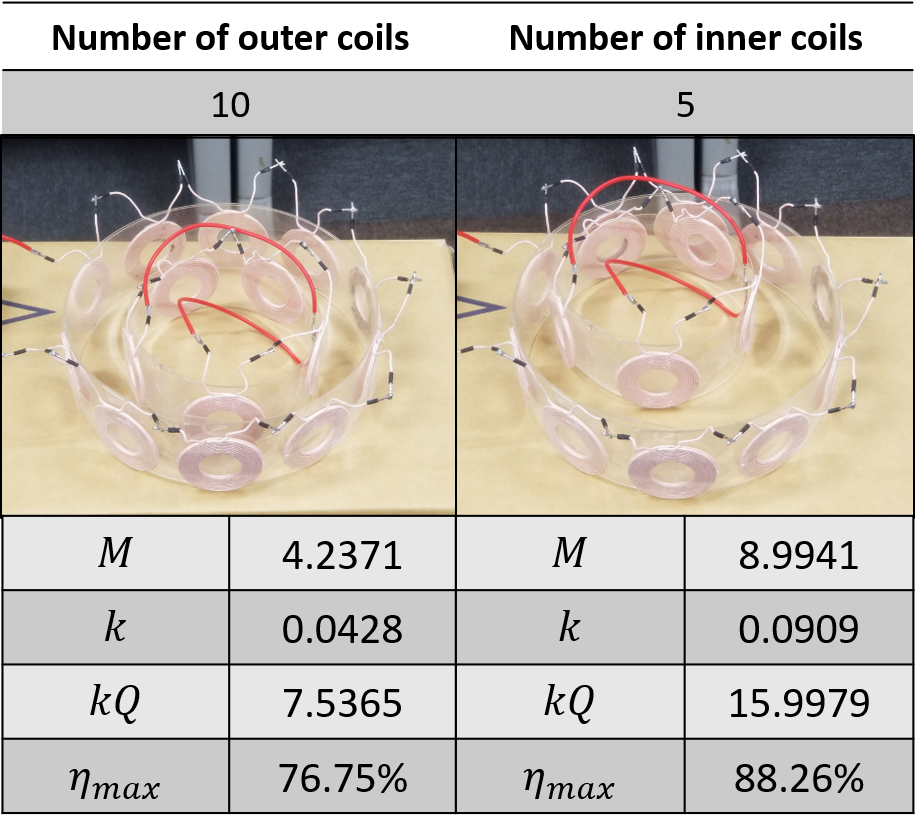
\includegraphics[width=0.6\linewidth]{images/4_coil_5_10_without_ferrite.png}
    \caption{Coil-array IPT structure (Both sides without ferrite tile), inner coil in the center of the outer coil (Left), inner coil next to the outer coil (Right).}
\end{figure}
\begin{figure}[htbp]
    \centering
    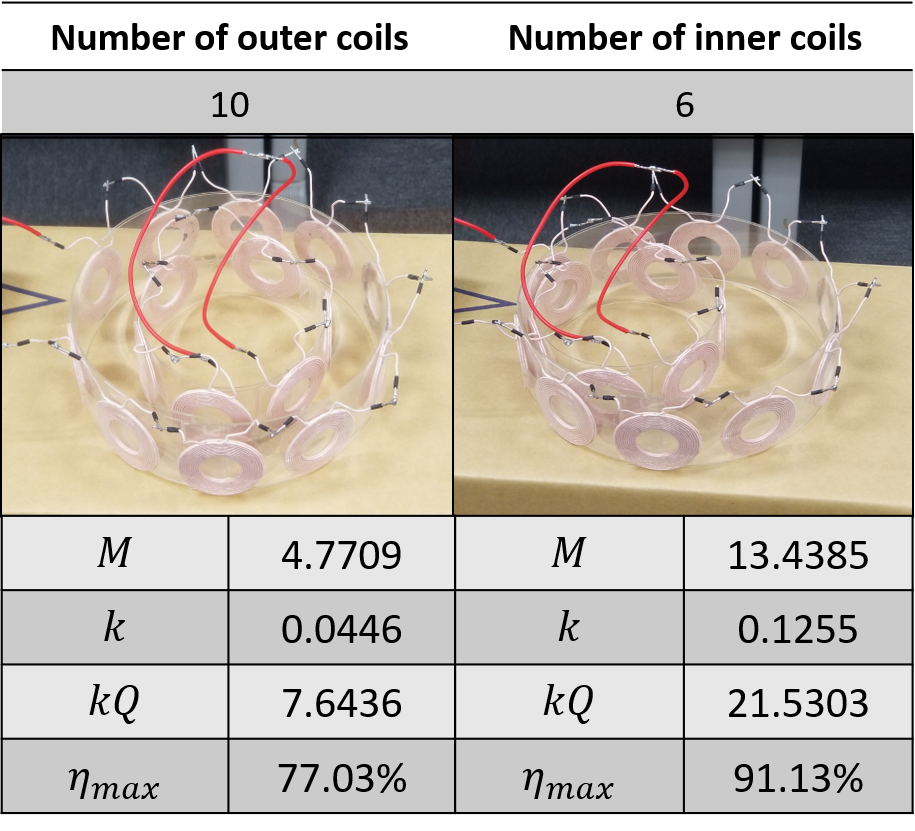
\includegraphics[width=0.6\linewidth]{images/4_coil_6_10_without_ferrite.png}
    \caption{Coil-array IPT structure (Both sides without ferrite tile), inner coil in the center of the outer coil (Left), inner coil next to the outer coil (Right).}
\end{figure}
\begin{figure}[htbp]
    \centering
    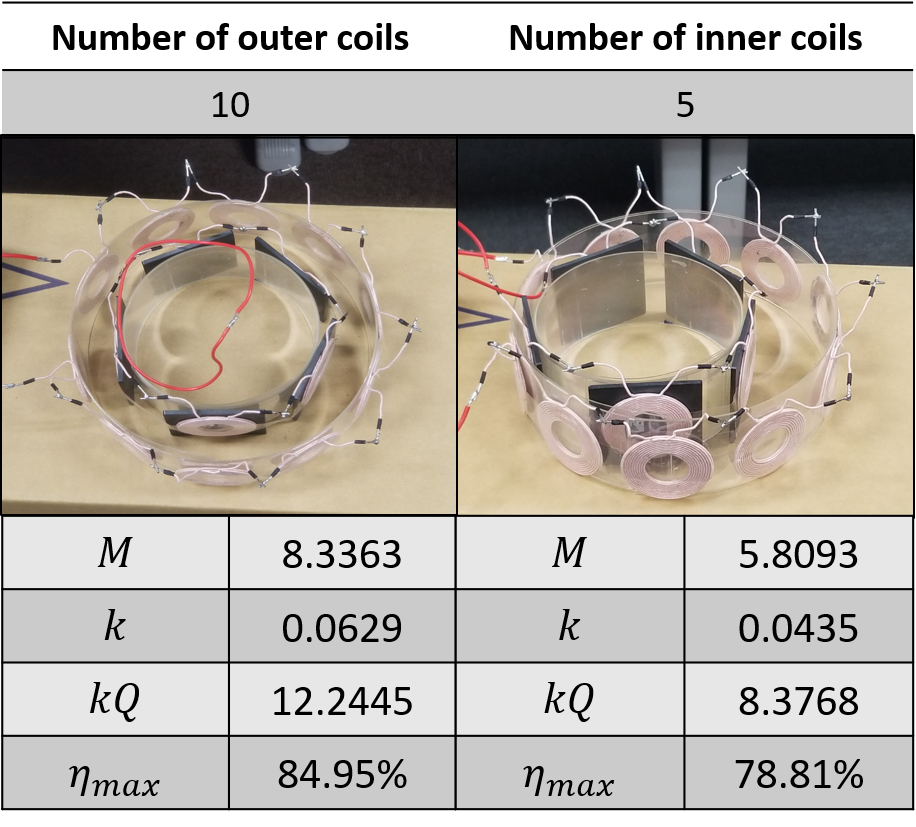
\includegraphics[width=0.6\linewidth]{images/4_coil_6_10_inner_with_ferrite.png}
    \caption{Coil-array IPT structure (Inner small coils with ferrite tile, outer small coils without ferrite tile), inner coil in the center of the outer coil (Left), inner coil next to the outer coil (Right).}
\end{figure}

\begin{table}[htbp]
    \centering
    \caption{Maximum power transfer efficiency of different coil arrangements.}
    \begin{tabular}{|>{\centering\arraybackslash}m{3.3cm}|>{\centering\arraybackslash}m{2.5cm}|>{\centering\arraybackslash}m{2.5cm}|>{\centering\arraybackslash}m{2.5cm}|>{\centering\arraybackslash}m{2.5cm}|}
        \hline
        \textbf{Shift}                                    & \textbf{Numbers of coil (Outer - Inner)} & \textbf{Both coils with ferrite} & \textbf{Both coils without ferrite} & \textbf{Outer coils without ferrite, inner coils with ferrite} \\ \hline
        \multirow{2}{3.3cm}{Inner coil in the center}         & 10 - 5                             & 78.41\%                          & 76.75\%                             & 84.95\%                            \\ \cline{2-5}
                                                          & 10 - 6                             &                                  & 77.03\%                             &                                    \\ \hline
        \multirow{2}{3.3cm}{Inner coil close to the one side} & 10 - 5                             &                                  & 88.26\%                             & 78.80\%                            \\ \cline{2-5}
                                                          & 10 - 6                             &                                  & 91.13\%                             &                                    \\ \hline
    \end{tabular}
\end{table}

\begin{itemize}
\item When we increase the number of inner coils, the maximum PTE (Power transfer efficiency) will increase.
\item If the numbers of outer and inner coils are the same, when outer coils without ferrite and inner coils with ferrite, we can get the maximum PTE.
\item When there is no ferrite outside the inner coil, the PTE will increase if the inner coil deviates from the middle, and vice versa.
\end{itemize}


\section{Coil array WPT under seawater}